%--------------------------------------------------------------------------------------------------------------------  
%--------------------------------------------------------------------------------------------------------------------


\subsection{Factibilidad tecnológica}  

  \newpage


%--------------------------------------------------------------------------------------------------------------------  
%--------------------------------------------------------------------------------------------------------------------

  \subsubsection{Propuesta de alternativas de diseño}  

  \newpage


%--------------------------------------------------------------------------------------------------------------------  
%--------------------------------------------------------------------------------------------------------------------

  \subsubsection{Elección de una solución}  

  \newpage


%--------------------------------------------------------------------------------------------------------------------  
%--------------------------------------------------------------------------------------------------------------------

  \subsubsection{DFMEA}  

  \newpage

%--------------------------------------------------------------------------------------------------------------------  
%--------------------------------------------------------------------------------------------------------------------

  \subsection{Factibilidad de tiempos. Planificación (PERT y simulación de Montecarlo) y programación (Gant). Análisis de Riesgos}  

  %--------------------------------------------------------------------------------------------------------------------  
  %--------------------------------------------------------------------------------------------------------------------

  \subsection{Factibilidad económica. (Mercado, costos, ciclo de vida, VAN, TIR)}  

  \subsubsection{Análisis de mercado}  

  Los nanomateriales poseen una gran potencialidad a nivel tecnológico, ya que posibilitan la optimización y mejora de actuales
  de materiales actuales.
  Particularmente utilizando el proceso de sinterizado de materiales magneticos se obtiene materiales
  con caracteristicas magneticas conciderablemente mejores que los materiales actualmente usados en la industria.
  Los materiales magneticos son de vital importancia el campo de la generación de energia electrica, almacenamiento electronico de datos, 
  desarrollo de sensores electrónico, etc.
  \newline

    \newpage
  %--------------------------------------------------------------------------------------------------------------------
  %--------------------------------------------------------------------------------------------------------------------

  \subsubsection{Análisis de la competencia}  

  \vspace{15px}
  %\begin{center}
  
\includegraphics[width=200px]{../../Documentacion/Diagramas/logo(1).jpg}
  % logo(1).jpg: 365x63 pixel, 72dpi, 12.88x2.22 cm, bb=0 0 365 63
  %\end{center}
  \vspace{25px}

  \begin{wrapfigure}{r}{0.55\textwidth}
  \vspace{-20px}  
  \begin{center}
    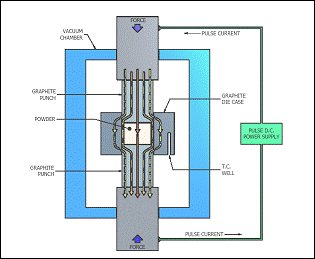
\includegraphics[width=0.4\textwidth]{../../Documentacion/Diagramas/image004.jpg}
  \end{center}
  \caption{SPS}
  \vspace{-20px}
  \end{wrapfigure}

  En el mercado encontramos soluciones de gran emplazamiento y envergadura, como lo son los propuestos por \href{''http://thermaltechnology.com/index.php?option=com_content&view=article&id=84''}{Thermal Technology LLC}
  basado en la tecnología de Spark Plasma Sintering (SPS) un revolucionario en polvo de alta velocidad de proceso de consolidación.
  SPS utiliza alto pulsos de alta corriente continua para activar la consolidación y la reacción de sinterización de los
  materiales. Un sistesma de SPS trabaja con materiales conductores, no conductores y compuesto a cualquier nivel de densidad.
  La ventaja de SPS es ahorro de tiempo y energía y la capacidad de retener nanoestructuras.


  %--------------------------------------------------------------------------------------------------------------------  
  %--------------------------------------------------------------------------------------------------------------------

  \subsubsection{Planes de crecimiento}  
  El proyecto en un principio propone realizar la automatización del proceso de sinterizado estableciendo las normas de seguidad
  que corresponden. En un segundo paso, realizar las medeciones sobre las mágnitudes involucradas en el proceso. Tensión, corriente
  tiempo de descarga, etc, y su posterior almacenamiento. Finalmente todo lo anterior se lo integraría de forma que pueda sincronizar
  contra un servidor en red.

  %--------------------------------------------------------------------------------------------------------------------  
  %--------------------------------------------------------------------------------------------------------------------

  \subsubsection{Objetivos de costo}  
  El objetivo propuesto trata de desarrollar instrumental de bajo o mediano costo en comparación a las opciones propuestas por
  la competencia. Desde ese punto de vista, el proceso de sinterizado a través de descarga de los capacitores propuesto es mas 
  eficiente

  %--------------------------------------------------------------------------------------------------------------------  
  %--------------------------------------------------------------------------------------------------------------------

  \newpage


%--------------------------------------------------------------------------------------------------------------------  
%--------------------------------------------------------------------------------------------------------------------

  \subsection{Factibilidad legal y responsabilidad civil (regulaciones y licencias}  

  \newpage


%--------------------------------------------------------------------------------------------------------------------  
%--------------------------------------------------------------------------------------------------------------------
